In this Chapter we use the constrained minimization problem put forth in Section \ref{sec:consmin} to numerically solve the equation of motion. This numerical solution provides further evidence for the existence of Q-Vortex solitons and the profiles allow us to better understand the nature of the objects.

\section{Finite Element Formalism}
As we saw in Chapter \ref{chap:qballs}, in particular Section \ref{sec:consmin} the constrained minimization approach to the problem is well defined because of the coercivity of the functional $I[\,\cdot\,]$ along with its lower semi-continuity. This means we can utilize it as a tool to numerically solve the equation of motion (\ref{eq:DE}) if we can reduce the infinite dimensional domain $W^{1,2}_0(0,R)$ to finite dimensional.

To attack this problem we will begin by taking a subspace $A\subset W^{1,2}_0(0,R)$ spanned by $n$ vectors $\{\psi_i\}_{i = 1}^n$. We take the $\psi$'s to be orthonormal with respect to the following inner product
\begin{equation}\label{eq:innerprod}
\langle\alpha,\beta\rangle\coloneqq 2\pi\int_0^P r\alpha\beta\dd{r}
\end{equation}
where $\alpha,\beta\in A$.
The form of (\ref{eq:innerprod}) is suggested by the Noether Charge we saw in Chapter \ref{chap:qballs} and $\langle\varphi,\varphi\rangle = \|\varphi\|^2$ corresponds to almost exactly the Noether Charge (\ref{eq:spincharge}). Using this this basis we approximate functions $f \in W_0^{1,2}(0, P)$ simply as a linear combinations
\begin{equation}\label{eq:approx}
f = \sum_{i = 1}^na_i\psi_i
\end{equation}
with all $a_i\in \mathbb{R}$. Inserting this approximation into our functional (\ref{eq:actionfunc}) we can define a new multivariable function
\begin{equation}\label{eq:objfun}
F(\mathbf{a}) \coloneqq I[f] = I\!\left[\sum_{i = 1}^na_i\psi_i\right]
\end{equation}
where $\mathbf{a} = (a_1, a_2,\ldots, a_n)^\intercal\in \mathbb{R}^n$ is called the variational vector. Now our problem of minimizing the action over an infinite dimensional function space becomes one of finite dimension. That is, now we want to minimize a multi-variable function $F:\mathbb{R}^n\to\mathbb{R}$ which is easy (most of the time) numerically. To further restrict our study we look for solutions with finite charge i.e.
\begin{equation}\label{eq:constraint}
\langle f, f \rangle = \|f\|^2 = J_0 < \infty.
\end{equation}
Upon inserting (\ref{eq:approx}) into (\ref{eq:constraint}) we obtain the following condition\footnote{using the fact that the inner product is linear in both entries, and the fact that the basis is orthonormal i.e., $\langle \psi_i,\psi_j\rangle = \delta_{ij}$.} on the variational vector $\mathbf{a}$.
\begin{equation}\label{eq:approxcons}
\sum_{i = 1}^na_i^2 = J_0 \iff \|\mathbf{a}\|^2_{\mathbb{R}^n} = J_0
\end{equation}
This condition realizes our problem now as a constrained minimization problem where, given solitonic charge $J_0$, we can find the solution if we minimize over all functions satisfying (\ref{eq:approxcons}). Written out, our problem (\ref{eq:consmin}) has been simplified to
\begin{equation}\label{eq:problem}
\mathbf{a}_{\min, J_0}\coloneqq \min_{\mathbf{a}\in\mathbb{R}^n}\left\{F(\mathbf{a}) \,\mid\, \|\mathbf{a}\|^2_{\mathbb{R}^n} = J_0\right\}.
\end{equation}
We have used the notation $\mathbf{a}_{\min, J_0}$ to mean the vector $\mathbf{a}$ that minimizes $F$ for a prescribed $J_0$.

Now we note two very important facts. First, $F$ is a continuous function. This can be seen by expanding (\ref{eq:objfun}) and writing it as a sum over the basis. Since the basis is known ahead of time this expansion yields a polynomial in the $a_i$'s and since it is a polynomial, it is clearly continuous. Second, the constraint (\ref{eq:approxcons}) defines a compact set, in particular a sphere of radius $\sqrt{J_0}$ centered at the origin. With a continuous function defined over a compact set, we know the minima must be attained and hence this problem is well defined and has a solution.


\section{Implementation}\label{sec:imp}
The code written to implement the constrained minimization problem (\ref{eq:problem}) was written in Python with use of NumPy and SciPy\footnote{Both of which are pronounced with a ``pi'' sound, not ``pee''. Num``pi'', not numpee please.}. We now explain, and ellucidate the process we used to obtain the numerical solutions.

We begin with NumPy arrays initialized to $\psi_i = \sin{\frac{i\pi x}{r_\text{max}}}$ with $i$ running in the set $\{1,2,\ldots, n\}$ before we orthonormalize them using the  the Gram-Schmidt Procedure, and the inner product given in (\ref{eq:innerprod}). All integration is handled using Simpson's Rule, and the \texttt{scipy.integrate.simps} built in function. In the plot below we see the result of Gram-Schmidt orthonormalization procedure under this inner product for a basis of size 10.
\begin{figure}[H]
\centering
  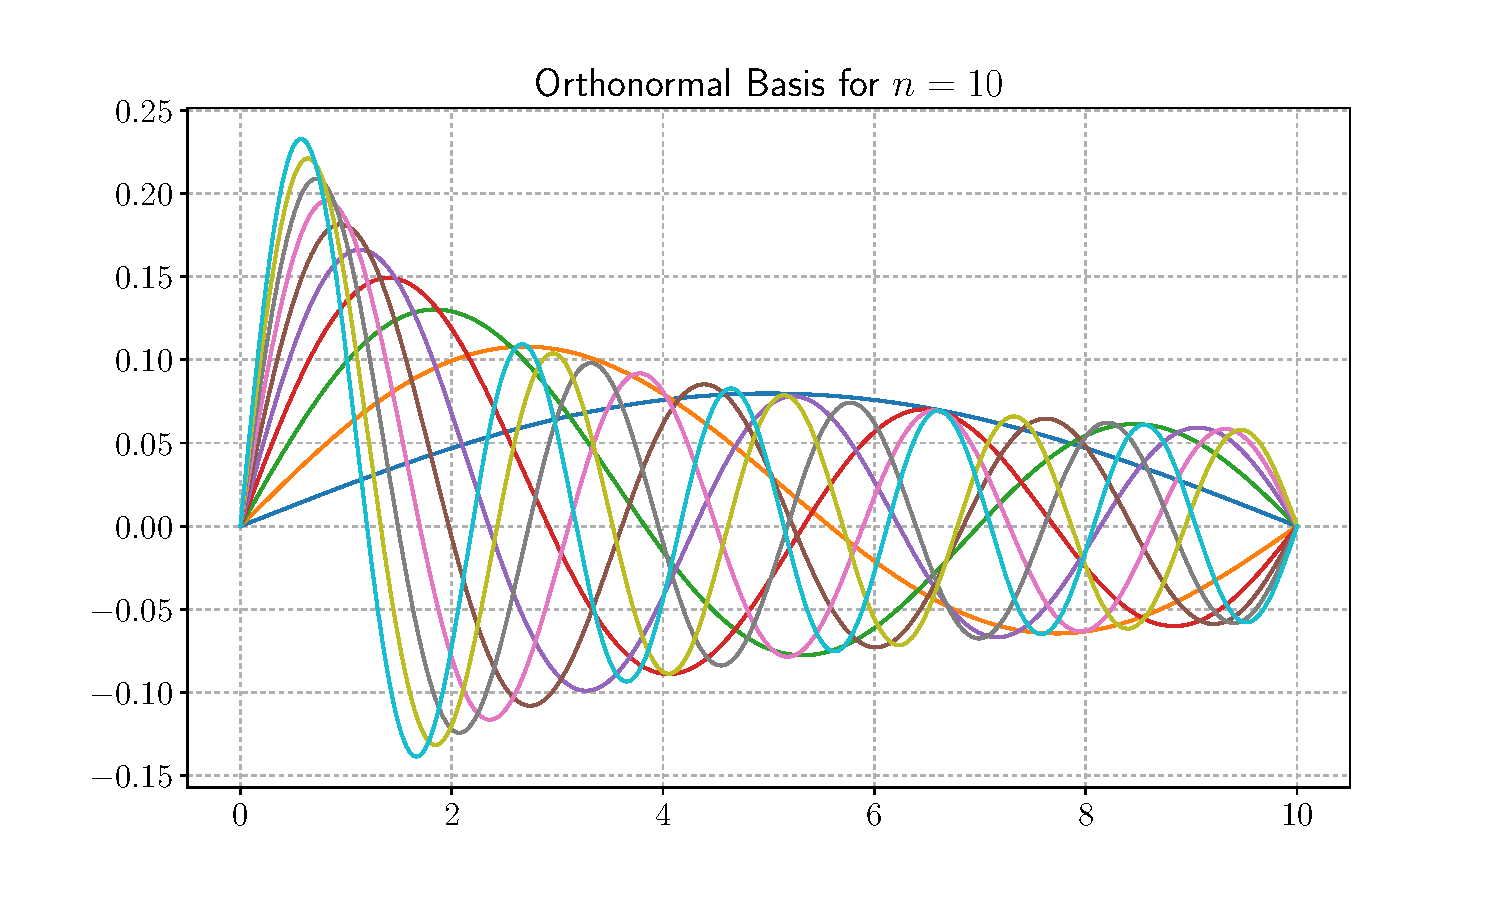
\includegraphics[width=0.95\linewidth]{basis.pdf}
  \caption{10 Orthonormal Basis Functions with $r_\text{max} = 10$}
  \label{fig:basis}
\end{figure}

With the basis at hand we can build the objective function (\ref{eq:objfun}), that is the function we wish to minimize. To satisfy (\ref{eq:approxcons}) we begin with the initial guess given by $\left(\sqrt{\frac{J_0}{n}}, \sqrt{\frac{J_0}{n}}, \ldots, \sqrt{\frac{J_0}{n}}\right)$. With an objective function, an initial guess, and a constraint, we can use SciPy's \texttt{scipy.optimize.minimize} to carry out the minimization\footnote{In order to have this function succeed for large values of $n$, that is a large basis set, the maximum number of iterations must be increased to reach the minimum.}. To reproduce the results in \cite{spinningq}, in particular, Figure 6, we chose parameters $a = 2, b = 1.1, \lambda = 1$ and with $J_0 = 30$ we obtain the following solution.
\begin{figure}[H]
\centering
  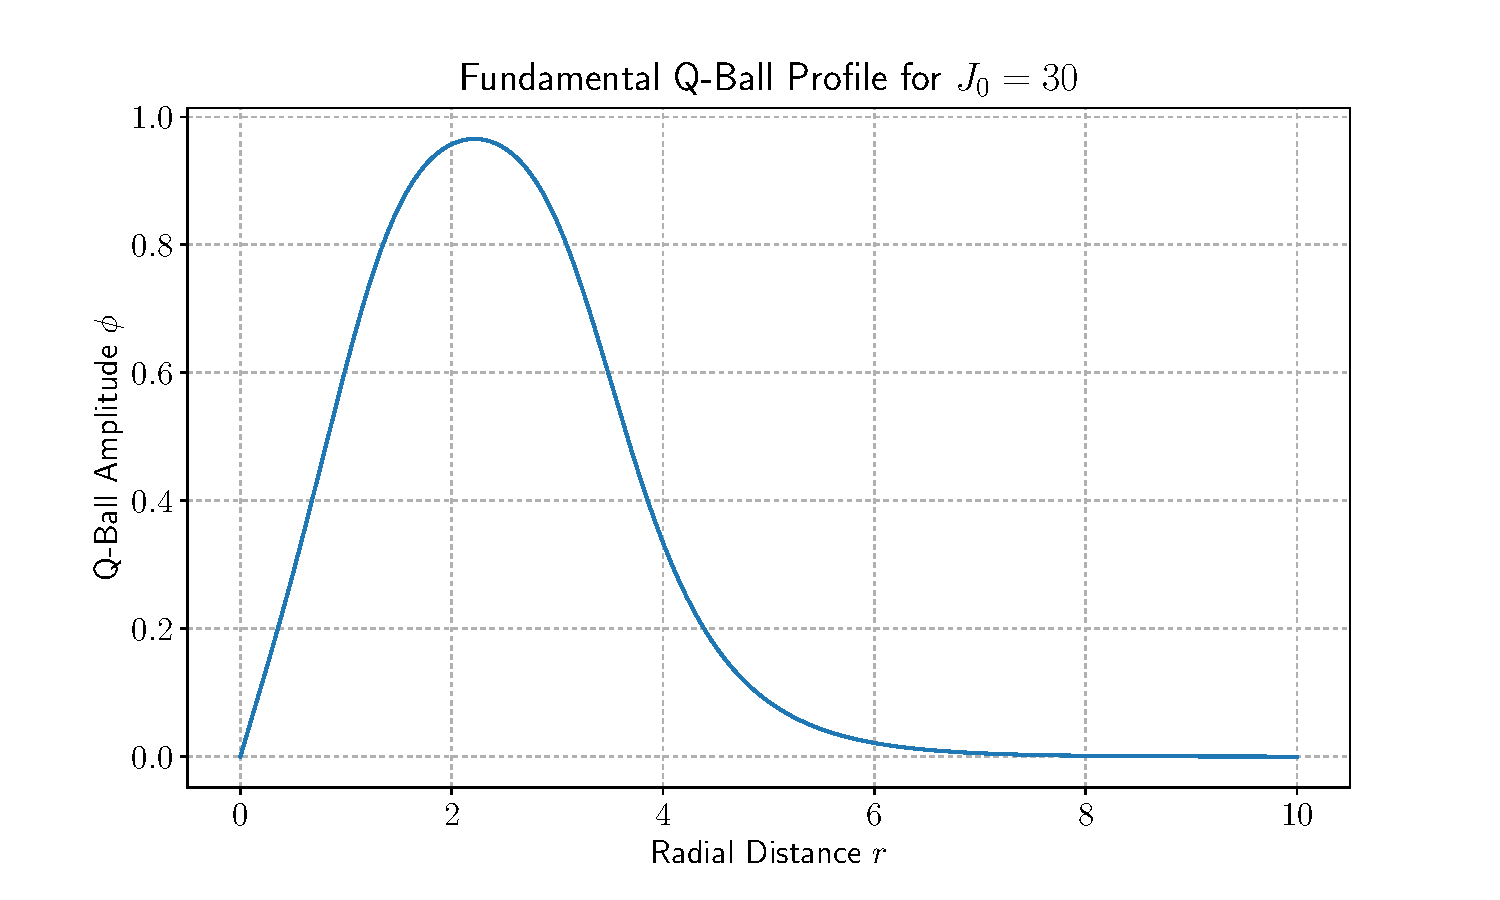
\includegraphics[width=0.95\linewidth]{qballprof30.pdf}
  \caption{$N = 1$ Excitation of Q-Vortex Solution}
  \label{fig:profile30}
\end{figure}
This plot was generated with 50 basis functions and an $x$-axis sampled 1000 times, i.e. $\dd{x} = 0.01$. With this solution we can then go on to calculate the Lagrange multiplier $\omega^2$ that we saw in Lemma \ref{lem:nonlineig}. To calculate $\omega^2$, we take the $\delta I$ and $\delta J$ as defined in Lemma \ref{lem:nonlineig}, and take the test function $\psi$ to be exactly $\phi$. This may seem like cheating, however $\delta I = \chi\delta J$ should hold for all $\psi$, and in particular $\psi = \phi$. We can then numerically calculate $\delta I$ and $\delta J$, calculate the Lagrange multiplier by taking the quotient $\chi = \frac{\delta I}{\delta J}$, and then using the relation $4\pi\chi = \omega^2$ we have $\omega = \sqrt{4\pi\chi}$. For the plot above this yields $\omega = 0.7216$.

We can then run this procedure for multiple values of $N$ to further understand how the Q-Vortex behaves with larger $N$ values. We note how, as we increase $N$, the peak of the soliton moves outward similar to how objects with more angular momentum tend to increase their radii.
\begin{figure}[H]
\centering
  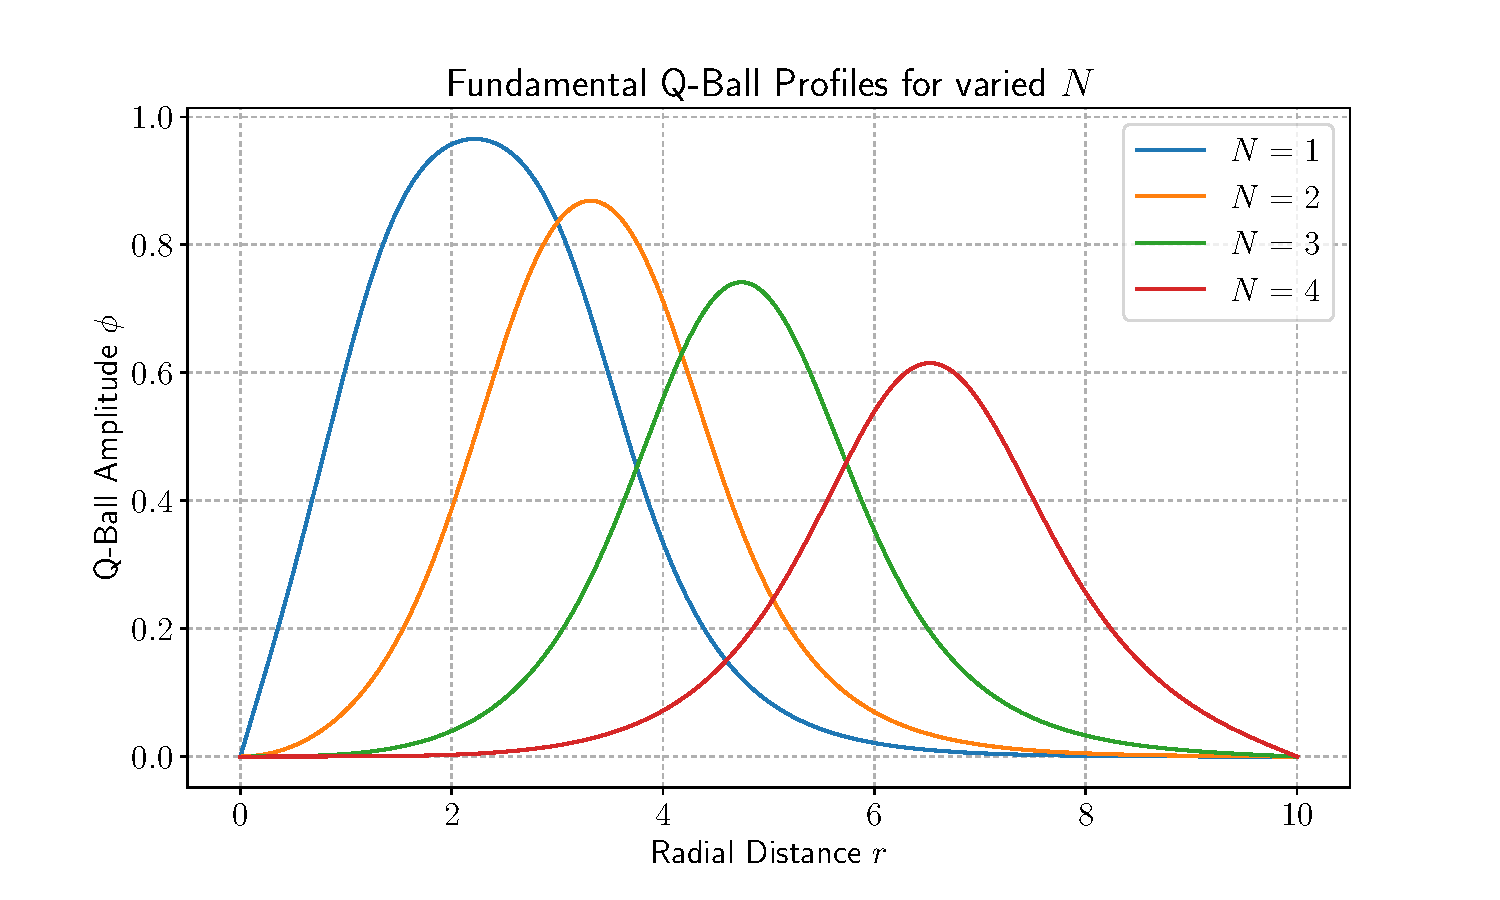
\includegraphics[width=0.95\linewidth]{qballprofs.pdf}
  \caption{First Four Fundamental Q-Vortex Solutions}
  \label{fig:profiles}
\end{figure}
Now that we have solutions at hand, it is important to understand the error associated with them. To measure the error we use the following idea and metric. If the solutions computed above are accurate, they should of course satisfy the equation of motion (\ref{eq:DE}). Thus we can add everything to one side, multiply by $r^2$, square the differential equation, and integrate\footnote{We multiply by $r^2$ to make our lives easier so we don't have to deal with the inverse powers of $r$ numerically.}.
\begin{equation}
\mathrm{error} = \int_0^R \left(r\left(r\phi_{r}\right)_r + \omega^2r^2\phi - N^2\phi - \lambda r^2\left(6\phi^5 - 4a\phi^3 + 2b\phi\right)\right)^2\dd{r}
\end{equation}
We can then tabulate the associated values for each solution shown in Figure \ref{fig:profiles}.
\begin{table}[H]
    \centering
    \begin{tabular}{| c | c | c |} \hline
    $N$ & $\omega$ & error \\ \hline
    1 & 0.72156 & 0.00626 \\ \hline
    2 & 0.85271 & 0.00084 \\ \hline
    3 & 1.01243 & 0.00021 \\ \hline
    4 & 1.16983 & 0.01622 \\ \hline
    \end{tabular}
    \caption{Parameters for $J_0 = 30$}
    \label{tab:params}
\end{table}

It is then natural to ask, for a given $N$, how does omega change as we vary the power $J_0$. Below we see that as the power is increased the soliton peak flattens and moves outward.
\begin{figure}[H]
\centering
  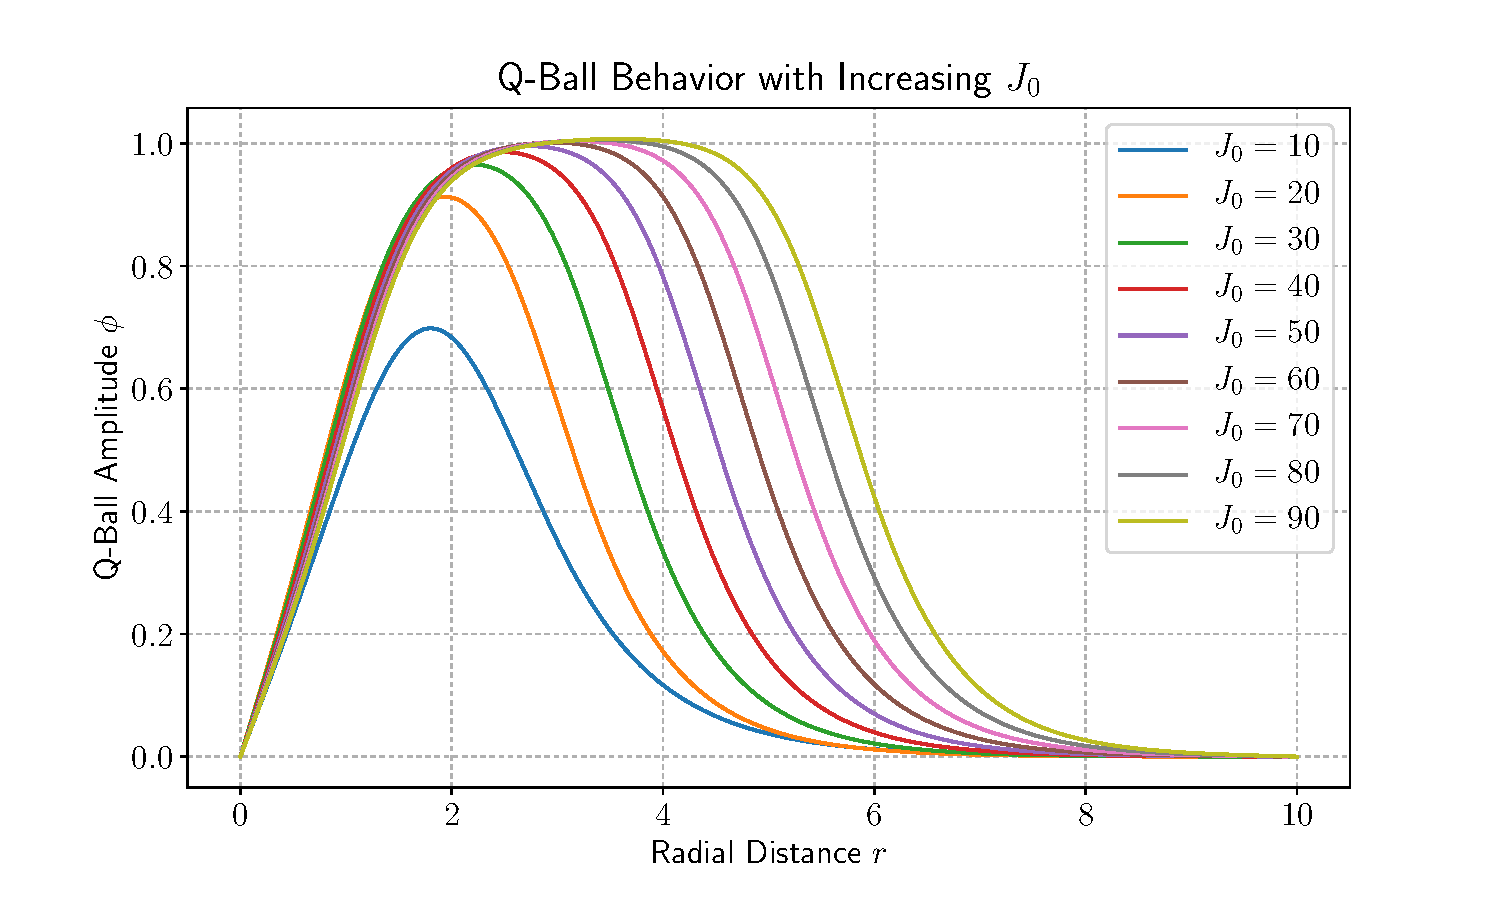
\includegraphics[width=0.95\linewidth]{varypower.pdf}
  \caption{Flat Top Emergence of Q-Vortex Soliton}
  \label{fig:flattops}
\end{figure}
The parameters for this plot is shown in the table below.
\begin{table}[H]
    \centering
    \begin{tabular}{| c | c | c |} \hline
    $J_0$ & $\omega$ & error \\ \hline
    10 & 1.06898 & 0.00002 \\ \hline
    20 & 0.80058 & 0.00498 \\ \hline
    30 & 0.72156 & 0.00626 \\ \hline
    40 & 0.68074 & 0.00137 \\ \hline
    50 & 0.65481 & 0.00447 \\ \hline
    60 & 0.63783 & 0.03409 \\ \hline
    70 & 0.62205 & 0.02264 \\ \hline
    80 & 0.61019 & 0.00427 \\ \hline
    90 & 0.60444 & 0.06596 \\ \hline
    \end{tabular}
    \caption{Parameters for $N = 1$}
    \label{tab:paramsN}
\end{table}
It is easy to see in this table that as the power increases, omega not  only decreases, but it looks as though it tends to some number. To investigate this further we performed a finer scan to understand how the power $J_0$ effects $\omega$.
\begin{figure}[H]
\centering
  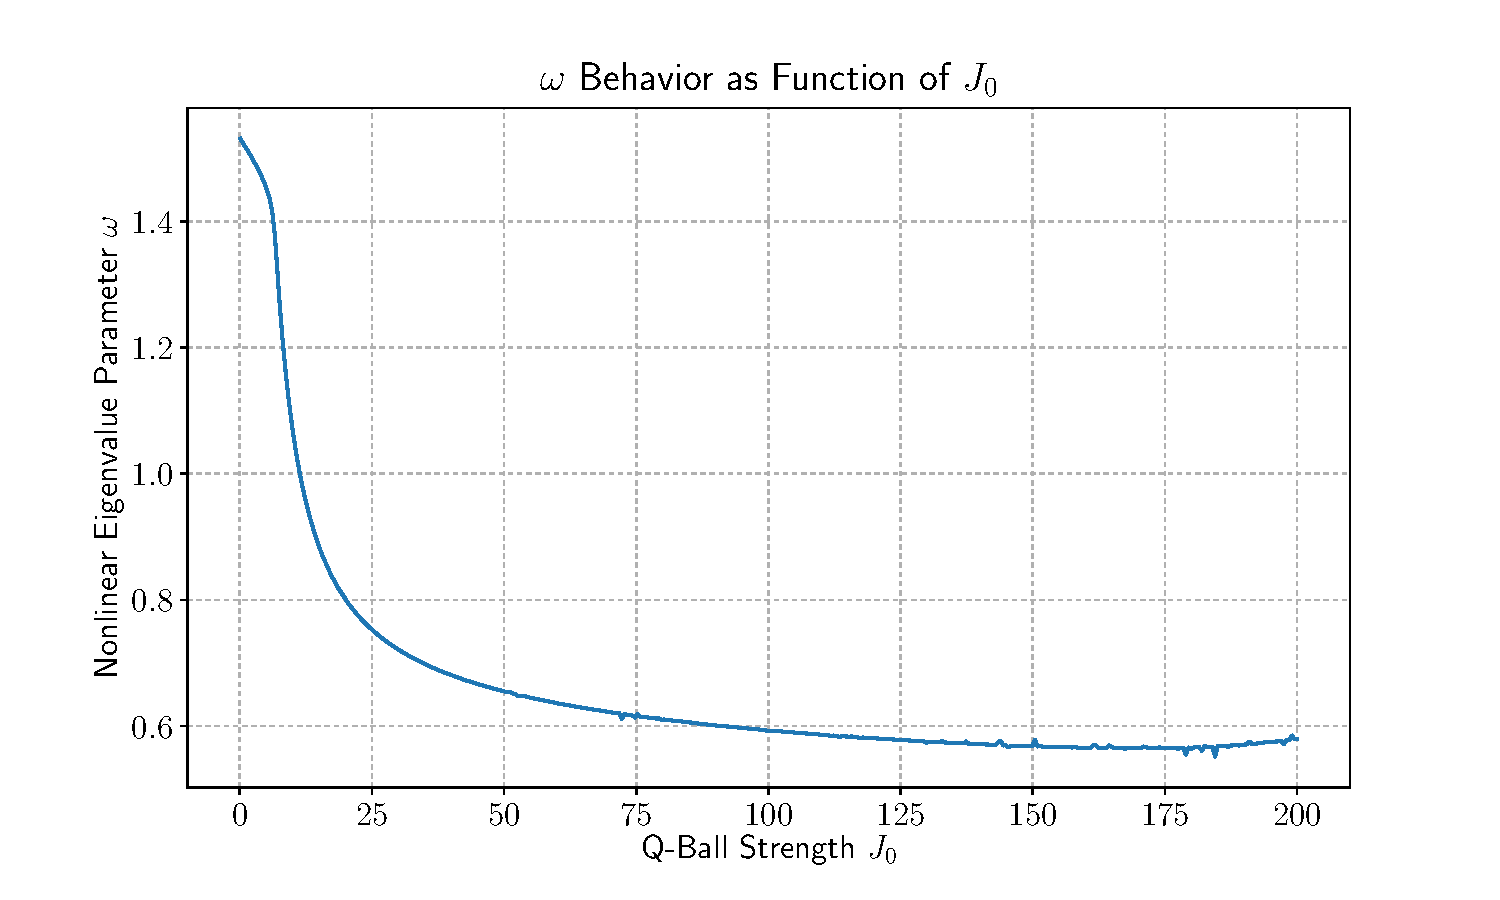
\includegraphics[width=0.95\linewidth]{omegavJ.pdf}
  \caption{$\omega$ vs. $J_0$ Parameter Space Scan}
  \label{fig:paramspace}
\end{figure}
As this plot shows, as we increase the $J_0$, $\omega$ falls very quickly at first, and then more slowly as it dips slightly below 0.6. In particular the minimum this curve achieves (not including small deviations) is roughly 0.57.





